\documentclass[twoside]{book}

% Packages required by doxygen
\usepackage{fixltx2e}
\usepackage{calc}
\usepackage{doxygen}
\usepackage[export]{adjustbox} % also loads graphicx
\usepackage{graphicx}
\usepackage[utf8]{inputenc}
\usepackage{makeidx}
\usepackage{multicol}
\usepackage{multirow}
\PassOptionsToPackage{warn}{textcomp}
\usepackage{textcomp}
\usepackage[nointegrals]{wasysym}
\usepackage[table]{xcolor}

% NLS support packages
\usepackage[ngerman]{babel}

% Font selection
\usepackage[T1]{fontenc}
\usepackage[scaled=.90]{helvet}
\usepackage{courier}
\usepackage{amssymb}
\usepackage{sectsty}
\renewcommand{\familydefault}{\sfdefault}
\allsectionsfont{%
  \fontseries{bc}\selectfont%
  \color{darkgray}%
}
\renewcommand{\DoxyLabelFont}{%
  \fontseries{bc}\selectfont%
  \color{darkgray}%
}
\newcommand{\+}{\discretionary{\mbox{\scriptsize$\hookleftarrow$}}{}{}}

% Page & text layout
\usepackage{geometry}
\geometry{%
  a4paper,%
  top=2.5cm,%
  bottom=2.5cm,%
  left=2.5cm,%
  right=2.5cm%
}
\tolerance=750
\hfuzz=15pt
\hbadness=750
\setlength{\emergencystretch}{15pt}
\setlength{\parindent}{0cm}
\setlength{\parskip}{3ex plus 2ex minus 2ex}
\makeatletter
\renewcommand{\paragraph}{%
  \@startsection{paragraph}{4}{0ex}{-1.0ex}{1.0ex}{%
    \normalfont\normalsize\bfseries\SS@parafont%
  }%
}
\renewcommand{\subparagraph}{%
  \@startsection{subparagraph}{5}{0ex}{-1.0ex}{1.0ex}{%
    \normalfont\normalsize\bfseries\SS@subparafont%
  }%
}
\makeatother

% Headers & footers
\usepackage{fancyhdr}
\pagestyle{fancyplain}
\fancyhead[LE]{\fancyplain{}{\bfseries\thepage}}
\fancyhead[CE]{\fancyplain{}{}}
\fancyhead[RE]{\fancyplain{}{\bfseries\leftmark}}
\fancyhead[LO]{\fancyplain{}{\bfseries\rightmark}}
\fancyhead[CO]{\fancyplain{}{}}
\fancyhead[RO]{\fancyplain{}{\bfseries\thepage}}
\fancyfoot[LE]{\fancyplain{}{}}
\fancyfoot[CE]{\fancyplain{}{}}
\fancyfoot[RE]{\fancyplain{}{\bfseries\scriptsize Erzeugt von Doxygen }}
\fancyfoot[LO]{\fancyplain{}{\bfseries\scriptsize Erzeugt von Doxygen }}
\fancyfoot[CO]{\fancyplain{}{}}
\fancyfoot[RO]{\fancyplain{}{}}
\renewcommand{\footrulewidth}{0.4pt}
\renewcommand{\chaptermark}[1]{%
  \markboth{#1}{}%
}
\renewcommand{\sectionmark}[1]{%
  \markright{\thesection\ #1}%
}

% Indices & bibliography
\usepackage{natbib}
\usepackage[titles]{tocloft}
\setcounter{tocdepth}{3}
\setcounter{secnumdepth}{5}
\makeindex

% Hyperlinks (required, but should be loaded last)
\usepackage{ifpdf}
\ifpdf
  \usepackage[pdftex,pagebackref=true]{hyperref}
\else
  \usepackage[ps2pdf,pagebackref=true]{hyperref}
\fi
\hypersetup{%
  colorlinks=true,%
  linkcolor=blue,%
  citecolor=blue,%
  unicode%
}

% Custom commands
\newcommand{\clearemptydoublepage}{%
  \newpage{\pagestyle{empty}\cleardoublepage}%
}

\usepackage{caption}
\captionsetup{labelsep=space,justification=centering,font={bf},singlelinecheck=off,skip=4pt,position=top}

%===== C O N T E N T S =====

\begin{document}

% Titlepage & ToC
\hypersetup{pageanchor=false,
             bookmarksnumbered=true,
             pdfencoding=unicode
            }
\pagenumbering{alph}
\begin{titlepage}
\vspace*{7cm}
\begin{center}%
{\Large E\+S\+P8266 Template }\\
\vspace*{1cm}
{\large Erzeugt von Doxygen 1.8.13}\\
\end{center}
\end{titlepage}
\clearemptydoublepage
\pagenumbering{roman}
\tableofcontents
\clearemptydoublepage
\pagenumbering{arabic}
\hypersetup{pageanchor=true}

%--- Begin generated contents ---
\chapter{Klassen-\/\+Verzeichnis}
\section{Auflistung der Klassen}
Hier folgt die Aufzählung aller Klassen, Strukturen, Varianten und Schnittstellen mit einer Kurzbeschreibung\+:\begin{DoxyCompactList}
\item\contentsline{section}{\hyperlink{class_a_p_i}{A\+PI} }{\pageref{class_a_p_i}}{}
\item\contentsline{section}{\hyperlink{class_auth}{Auth} }{\pageref{class_auth}}{}
\item\contentsline{section}{\hyperlink{class_clock}{Clock} }{\pageref{class_clock}}{}
\item\contentsline{section}{\hyperlink{class_controller}{Controller} }{\pageref{class_controller}}{}
\item\contentsline{section}{\hyperlink{class_e_s_p___tools}{E\+S\+P\+\_\+\+Tools} }{\pageref{class_e_s_p___tools}}{}
\item\contentsline{section}{\hyperlink{class_f_f_s}{F\+FS} }{\pageref{class_f_f_s}}{}
\item\contentsline{section}{\hyperlink{class_f_f_sjson_file}{F\+F\+Sjson\+File} }{\pageref{class_f_f_sjson_file}}{}
\item\contentsline{section}{\hyperlink{class_f_f_sstring_file}{F\+F\+Sstring\+File} }{\pageref{class_f_f_sstring_file}}{}
\item\contentsline{section}{\hyperlink{class_i2_c}{I2C} }{\pageref{class_i2_c}}{}
\item\contentsline{section}{\hyperlink{class_l_c_d}{L\+CD} }{\pageref{class_l_c_d}}{}
\item\contentsline{section}{\hyperlink{class_l_o_g_g_i_n_g}{L\+O\+G\+G\+I\+NG} }{\pageref{class_l_o_g_g_i_n_g}}{}
\item\contentsline{section}{\hyperlink{class_m_q_t_t}{M\+Q\+TT} }{\pageref{class_m_q_t_t}}{}
\item\contentsline{section}{\hyperlink{class_o_w_i_r_e}{O\+W\+I\+RE} }{\pageref{class_o_w_i_r_e}}{}
\item\contentsline{section}{\hyperlink{class_session}{Session} }{\pageref{class_session}}{}
\item\contentsline{section}{\hyperlink{class_sys_utils}{Sys\+Utils} }{\pageref{class_sys_utils}}{}
\item\contentsline{section}{\hyperlink{class_topic}{Topic} }{\pageref{class_topic}}{}
\item\contentsline{section}{\hyperlink{struct_t_topic}{T\+Topic} }{\pageref{struct_t_topic}}{}
\item\contentsline{section}{\hyperlink{class_w_e_b_i_f}{W\+E\+B\+IF} }{\pageref{class_w_e_b_i_f}}{}
\item\contentsline{section}{\hyperlink{class_w_i_f_i}{W\+I\+FI} }{\pageref{class_w_i_f_i}}{}
\end{DoxyCompactList}

\chapter{Klassen-\/\+Dokumentation}
\hypertarget{class_a_p_i}{}\section{A\+PI Klassenreferenz}
\label{class_a_p_i}\index{A\+PI@{A\+PI}}


Zusammengehörigkeiten von A\+PI\+:
\nopagebreak
\begin{figure}[H]
\begin{center}
\leavevmode
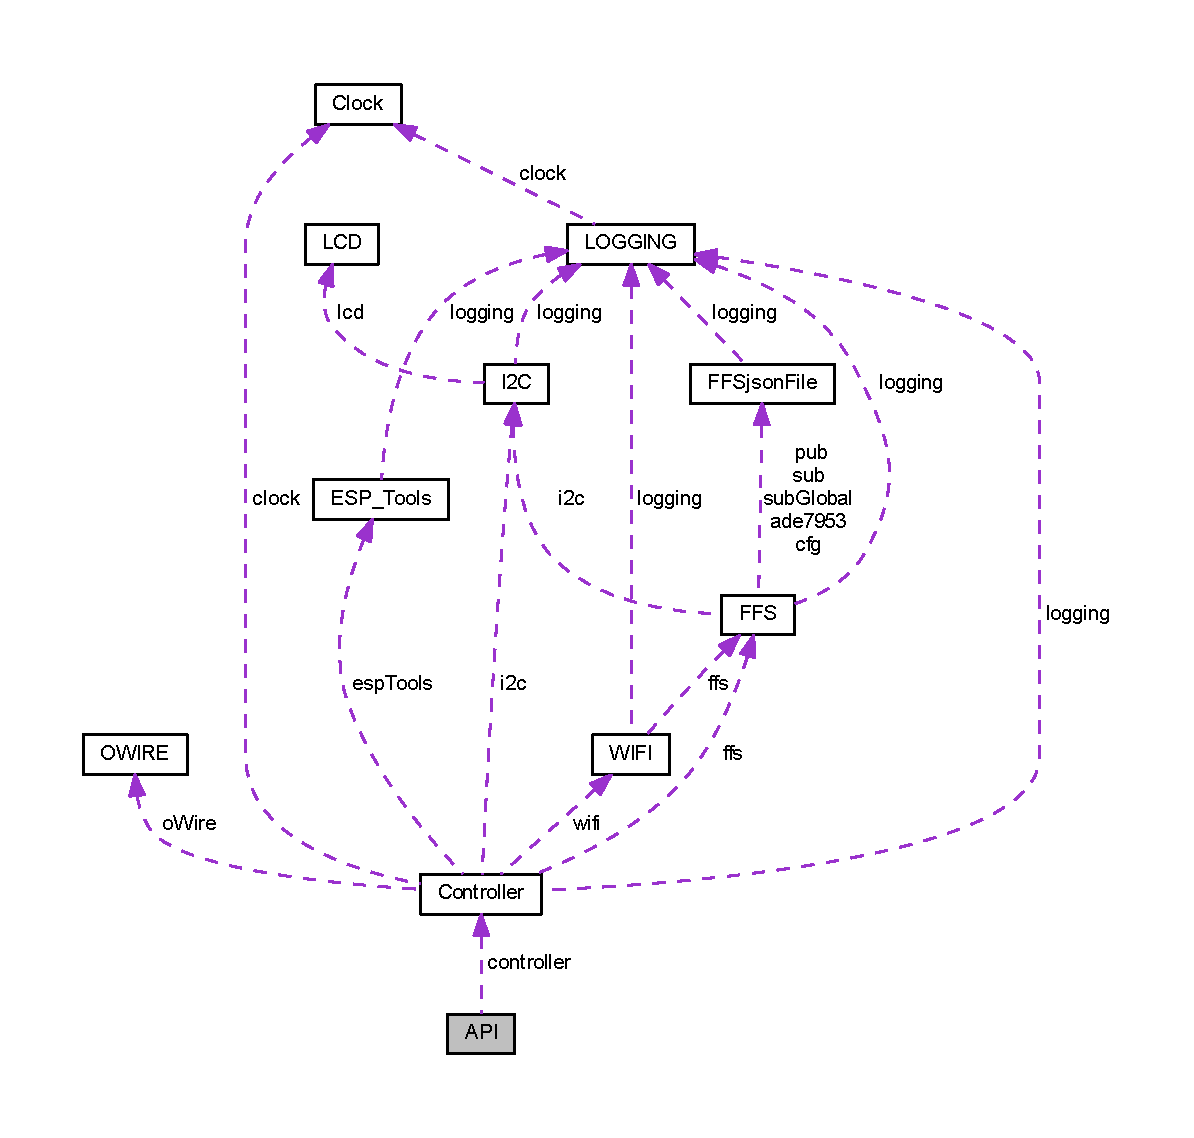
\includegraphics[width=350pt]{class_a_p_i__coll__graph}
\end{center}
\end{figure}
\subsection*{Öffentliche Methoden}
\begin{DoxyCompactItemize}
\item 
\mbox{\Hypertarget{class_a_p_i_a27a09222e98a84f49cf49e5c085fbe3d}\label{class_a_p_i_a27a09222e98a84f49cf49e5c085fbe3d}} 
{\bfseries A\+PI} (\hyperlink{class_controller}{Controller} \&controller)
\item 
\mbox{\Hypertarget{class_a_p_i_a2153db9ccf3b54c5fa9b885492a3b0e0}\label{class_a_p_i_a2153db9ccf3b54c5fa9b885492a3b0e0}} 
void {\bfseries start} ()
\item 
\mbox{\Hypertarget{class_a_p_i_afebdcc5458f58678900420e2be8990c6}\label{class_a_p_i_afebdcc5458f58678900420e2be8990c6}} 
String {\bfseries call} (\hyperlink{class_topic}{Topic} \&topic)
\item 
\mbox{\Hypertarget{class_a_p_i_a39ff2d68c232fd788fd16284b653eef5}\label{class_a_p_i_a39ff2d68c232fd788fd16284b653eef5}} 
String {\bfseries call} (String topics\+Args)
\item 
\mbox{\Hypertarget{class_a_p_i_a9fdc8dacbf201cfc8f7f9f2ecee8da59}\label{class_a_p_i_a9fdc8dacbf201cfc8f7f9f2ecee8da59}} 
String {\bfseries call} (string topics\+Args)
\item 
\mbox{\Hypertarget{class_a_p_i_aa53d4a4d6c09911634e8a82562a8f8a7}\label{class_a_p_i_aa53d4a4d6c09911634e8a82562a8f8a7}} 
void {\bfseries info} (const String \&msg)
\item 
\mbox{\Hypertarget{class_a_p_i_ab8497c19f62a12e9f4f7ea7e2308fe8f}\label{class_a_p_i_ab8497c19f62a12e9f4f7ea7e2308fe8f}} 
void {\bfseries error} (const String \&msg)
\item 
\mbox{\Hypertarget{class_a_p_i_a1f500c0f1d811e0f510f706e2cfd85c6}\label{class_a_p_i_a1f500c0f1d811e0f510f706e2cfd85c6}} 
void {\bfseries debug} (const String \&msg)
\end{DoxyCompactItemize}
\subsection*{Öffentliche Attribute}
\begin{DoxyCompactItemize}
\item 
\mbox{\Hypertarget{class_a_p_i_a940cddbb9d7df3506211ebe47f267cb3}\label{class_a_p_i_a940cddbb9d7df3506211ebe47f267cb3}} 
\hyperlink{class_controller}{Controller} \& {\bfseries controller}
\end{DoxyCompactItemize}


Die Dokumentation für diese Klasse wurde erzeugt aufgrund der Dateien\+:\begin{DoxyCompactItemize}
\item 
C\+:/\+T\+E\+M\+P/\+A\+D\+E7953-\/\+Power\+Socket/src/A\+P\+I.\+h\item 
C\+:/\+T\+E\+M\+P/\+A\+D\+E7953-\/\+Power\+Socket/src/A\+P\+I.\+cpp\end{DoxyCompactItemize}

\hypertarget{class_auth}{}\section{Auth Klassenreferenz}
\label{class_auth}\index{Auth@{Auth}}
\subsection*{Öffentliche Methoden}
\begin{DoxyCompactItemize}
\item 
\mbox{\Hypertarget{class_auth_a372114e80d70a2649df5c713a643022b}\label{class_auth_a372114e80d70a2649df5c713a643022b}} 
{\bfseries Auth} (\hyperlink{class_a_p_i}{A\+PI} \&api)
\item 
\mbox{\Hypertarget{class_auth_a426f6d69c1cc679442add50e0e167030}\label{class_auth_a426f6d69c1cc679442add50e0e167030}} 
void {\bfseries reset} ()
\item 
\mbox{\Hypertarget{class_auth_a435a805d8de617fc0031996da58919c1}\label{class_auth_a435a805d8de617fc0031996da58919c1}} 
bool {\bfseries check\+Password} (String username, String password)
\item 
\mbox{\Hypertarget{class_auth_ae142f6d59d2230dae2ca4997f9946b8e}\label{class_auth_ae142f6d59d2230dae2ca4997f9946b8e}} 
\hyperlink{class_session}{Session\+Ptr} {\bfseries create\+Session} (String username)
\item 
\mbox{\Hypertarget{class_auth_a8c3c138dedb562ab06f54270d42aaa6b}\label{class_auth_a8c3c138dedb562ab06f54270d42aaa6b}} 
\hyperlink{class_session}{Session\+Ptr} {\bfseries get\+Session} (String session\+Id)
\item 
\mbox{\Hypertarget{class_auth_a411c5a172f77139388a9d047027dfad4}\label{class_auth_a411c5a172f77139388a9d047027dfad4}} 
void {\bfseries delete\+Session} (String session\+Id)
\end{DoxyCompactItemize}


Die Dokumentation für diese Klasse wurde erzeugt aufgrund der Dateien\+:\begin{DoxyCompactItemize}
\item 
C\+:/\+T\+E\+M\+P/\+A\+D\+E7953-\/\+Power\+Socket/src/Auth.\+h\item 
C\+:/\+T\+E\+M\+P/\+A\+D\+E7953-\/\+Power\+Socket/src/Auth.\+cpp\end{DoxyCompactItemize}

\hypertarget{class_clock}{}\section{Clock Klassenreferenz}
\label{class_clock}\index{Clock@{Clock}}
\subsection*{Öffentliche Methoden}
\begin{DoxyCompactItemize}
\item 
\mbox{\Hypertarget{class_clock_a8a050959dcff11c85d695989e9099a8c}\label{class_clock_a8a050959dcff11c85d695989e9099a8c}} 
void {\bfseries start} ()
\item 
\mbox{\Hypertarget{class_clock_a90f110eacc7a87ce572dc1f2af77e25d}\label{class_clock_a90f110eacc7a87ce572dc1f2af77e25d}} 
void {\bfseries start} (const char $\ast$pool\+Server\+Name, int time\+Offset, int update\+Interval)
\item 
\mbox{\Hypertarget{class_clock_a0b77c3e7f33eb7ae0f018e469d96a250}\label{class_clock_a0b77c3e7f33eb7ae0f018e469d96a250}} 
void {\bfseries stop} ()
\item 
\mbox{\Hypertarget{class_clock_ae7c6708cf04b233655b501a97bb1e802}\label{class_clock_ae7c6708cf04b233655b501a97bb1e802}} 
void {\bfseries update} ()
\item 
\mbox{\Hypertarget{class_clock_a9df252eb56b672532a02e367a196c8a5}\label{class_clock_a9df252eb56b672532a02e367a196c8a5}} 
void {\bfseries force\+Update} ()
\item 
\mbox{\Hypertarget{class_clock_aa8504c02bd77bac45b0cdbb377b0ccd3}\label{class_clock_aa8504c02bd77bac45b0cdbb377b0ccd3}} 
time\+\_\+t {\bfseries now} ()
\item 
\mbox{\Hypertarget{class_clock_a8d7762e8bc2edd4e1da23a4db154f2c3}\label{class_clock_a8d7762e8bc2edd4e1da23a4db154f2c3}} 
String {\bfseries set} (\hyperlink{class_topic}{Topic} \&topic)
\item 
\mbox{\Hypertarget{class_clock_a0241ebe5ed63778f1135b12f669a16ee}\label{class_clock_a0241ebe5ed63778f1135b12f669a16ee}} 
String {\bfseries get} (\hyperlink{class_topic}{Topic} \&topic)
\item 
\mbox{\Hypertarget{class_clock_a0cfec3d5b76b22f96fb012c6dc64ac1e}\label{class_clock_a0cfec3d5b76b22f96fb012c6dc64ac1e}} 
String {\bfseries root} ()
\end{DoxyCompactItemize}


Die Dokumentation für diese Klasse wurde erzeugt aufgrund der Dateien\+:\begin{DoxyCompactItemize}
\item 
C\+:/\+T\+E\+M\+P/\+A\+D\+E7953-\/\+Power\+Socket/src/Clock.\+h\item 
C\+:/\+T\+E\+M\+P/\+A\+D\+E7953-\/\+Power\+Socket/src/Clock.\+cpp\end{DoxyCompactItemize}

\hypertarget{class_controller}{}\section{Controller Klassenreferenz}
\label{class_controller}\index{Controller@{Controller}}


Zusammengehörigkeiten von Controller\+:
\nopagebreak
\begin{figure}[H]
\begin{center}
\leavevmode
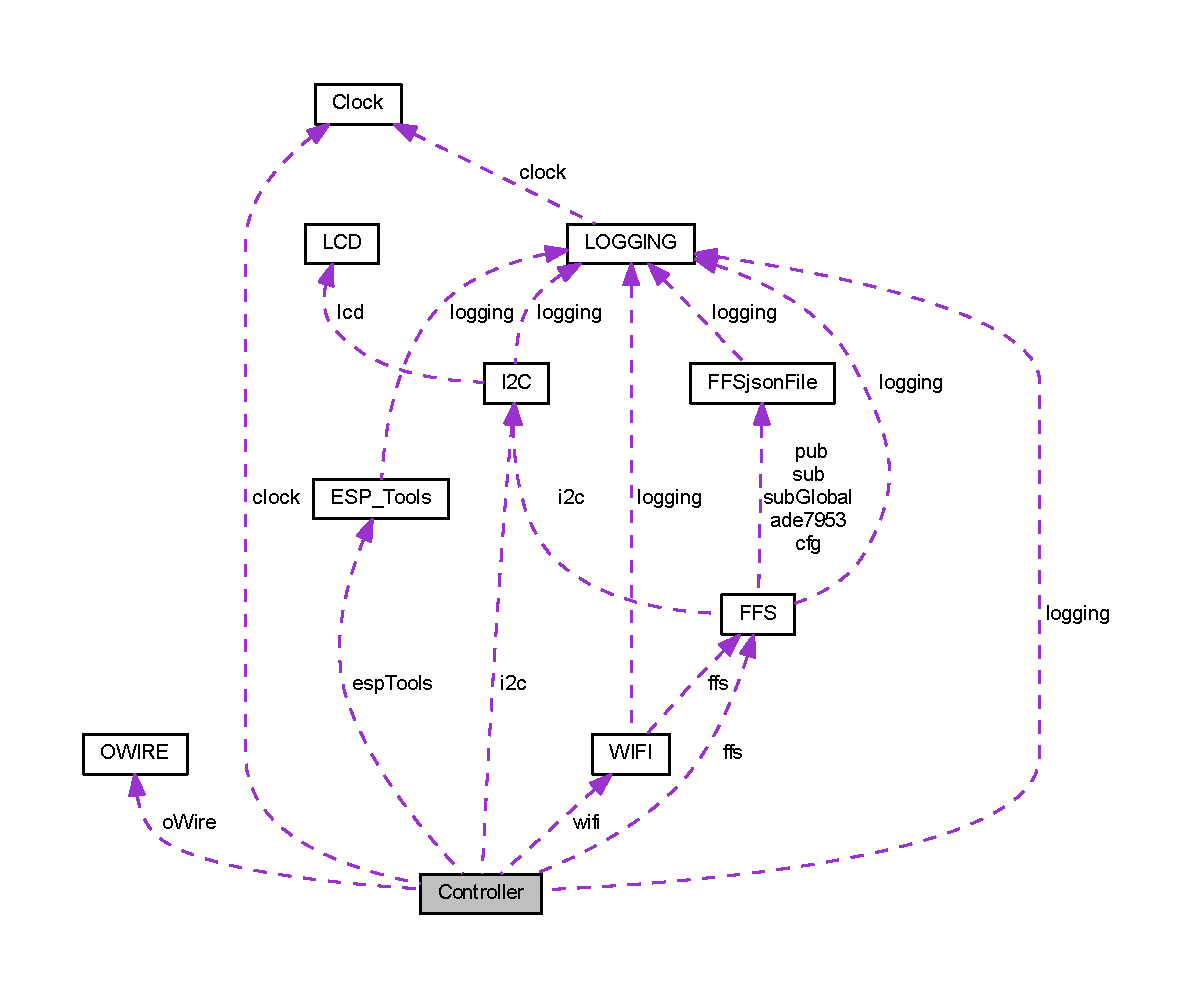
\includegraphics[width=350pt]{class_controller__coll__graph}
\end{center}
\end{figure}
\subsection*{Öffentliche Methoden}
\begin{DoxyCompactItemize}
\item 
\mbox{\Hypertarget{class_controller_ad535ad74055e645b7f44b7feeb4e82a8}\label{class_controller_ad535ad74055e645b7f44b7feeb4e82a8}} 
void {\bfseries start} ()
\item 
\mbox{\Hypertarget{class_controller_a0fee459be90ca9573b17fca3c8a87efe}\label{class_controller_a0fee459be90ca9573b17fca3c8a87efe}} 
void {\bfseries handle} ()
\item 
\mbox{\Hypertarget{class_controller_a40794552e89c83c124e15d73f7e0a21e}\label{class_controller_a40794552e89c83c124e15d73f7e0a21e}} 
void {\bfseries on\+\_\+wifi\+Connected} ()
\item 
\mbox{\Hypertarget{class_controller_aa9db3dcb8cdbef1d64724354a233848c}\label{class_controller_aa9db3dcb8cdbef1d64724354a233848c}} 
void {\bfseries on\+\_\+wifi\+Disconnected} ()
\item 
\mbox{\Hypertarget{class_controller_a806760bd84d31ee8caf2a51e160f950c}\label{class_controller_a806760bd84d31ee8caf2a51e160f950c}} 
String {\bfseries call} (\hyperlink{class_topic}{Topic} \&topic)
\item 
\mbox{\Hypertarget{class_controller_a2dbae78c843af54bee52c6d6ffcb2844}\label{class_controller_a2dbae78c843af54bee52c6d6ffcb2844}} 
void {\bfseries t\+\_\+1s\+\_\+\+Update} ()
\item 
\mbox{\Hypertarget{class_controller_ae801dc4b04a716949b296819e02c04f0}\label{class_controller_ae801dc4b04a716949b296819e02c04f0}} 
void {\bfseries t\+\_\+short\+\_\+\+Update} ()
\item 
\mbox{\Hypertarget{class_controller_adf58976c2adf11a541e0a7ad7ba653ef}\label{class_controller_adf58976c2adf11a541e0a7ad7ba653ef}} 
void {\bfseries t\+\_\+long\+\_\+\+Update} ()
\end{DoxyCompactItemize}
\subsection*{Öffentliche Attribute}
\begin{DoxyCompactItemize}
\item 
\mbox{\Hypertarget{class_controller_a55147b5c14f76de55eb646d25ccb746f}\label{class_controller_a55147b5c14f76de55eb646d25ccb746f}} 
\hyperlink{class_clock}{Clock} {\bfseries clock}
\item 
\mbox{\Hypertarget{class_controller_ad7e78721b65f5ed9000e090e818cf842}\label{class_controller_ad7e78721b65f5ed9000e090e818cf842}} 
\hyperlink{class_l_o_g_g_i_n_g}{L\+O\+G\+G\+I\+NG} {\bfseries logging}
\item 
\mbox{\Hypertarget{class_controller_a01b1677a2b304ddd3adb7410a18490f8}\label{class_controller_a01b1677a2b304ddd3adb7410a18490f8}} 
\hyperlink{class_f_f_s}{F\+FS} {\bfseries ffs}
\item 
\mbox{\Hypertarget{class_controller_a53536b2aadd851baf07052b861b5067d}\label{class_controller_a53536b2aadd851baf07052b861b5067d}} 
\hyperlink{class_w_i_f_i}{W\+I\+FI} {\bfseries wifi}
\item 
\mbox{\Hypertarget{class_controller_a52b5973eba6bacfcc2529559065b5415}\label{class_controller_a52b5973eba6bacfcc2529559065b5415}} 
\hyperlink{class_i2_c}{I2C} {\bfseries i2c}
\item 
\mbox{\Hypertarget{class_controller_a10065bc74597d961faef1dbece078862}\label{class_controller_a10065bc74597d961faef1dbece078862}} 
\hyperlink{class_o_w_i_r_e}{O\+W\+I\+RE} {\bfseries o\+Wire}
\item 
\mbox{\Hypertarget{class_controller_ae9e79871b8732041da577b81ce165ecf}\label{class_controller_ae9e79871b8732041da577b81ce165ecf}} 
\hyperlink{class_e_s_p___tools}{E\+S\+P\+\_\+\+Tools} {\bfseries esp\+Tools}
\end{DoxyCompactItemize}


Die Dokumentation für diese Klasse wurde erzeugt aufgrund der Dateien\+:\begin{DoxyCompactItemize}
\item 
C\+:/\+T\+E\+M\+P/\+A\+D\+E7953-\/\+Power\+Socket/src/Controller.\+h\item 
C\+:/\+T\+E\+M\+P/\+A\+D\+E7953-\/\+Power\+Socket/src/Controller.\+cpp\end{DoxyCompactItemize}

\hypertarget{class_e_s_p___tools}{}\section{E\+S\+P\+\_\+\+Tools Klassenreferenz}
\label{class_e_s_p___tools}\index{E\+S\+P\+\_\+\+Tools@{E\+S\+P\+\_\+\+Tools}}


Zusammengehörigkeiten von E\+S\+P\+\_\+\+Tools\+:
\nopagebreak
\begin{figure}[H]
\begin{center}
\leavevmode
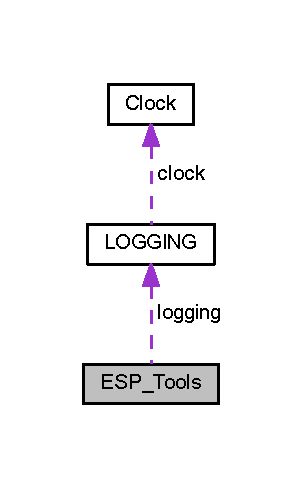
\includegraphics[width=147pt]{class_e_s_p___tools__coll__graph}
\end{center}
\end{figure}
\subsection*{Öffentliche Methoden}
\begin{DoxyCompactItemize}
\item 
\mbox{\Hypertarget{class_e_s_p___tools_a70230375980fbcb6b5154b9e87d0f617}\label{class_e_s_p___tools_a70230375980fbcb6b5154b9e87d0f617}} 
{\bfseries E\+S\+P\+\_\+\+Tools} (\hyperlink{class_l_o_g_g_i_n_g}{L\+O\+G\+G\+I\+NG} \&logging)
\item 
\mbox{\Hypertarget{class_e_s_p___tools_af6a83ab4830f92bd5bf0b1460a7a1553}\label{class_e_s_p___tools_af6a83ab4830f92bd5bf0b1460a7a1553}} 
void {\bfseries start} ()
\item 
\mbox{\Hypertarget{class_e_s_p___tools_af58fdfd7804981844fbf07e141e396b0}\label{class_e_s_p___tools_af58fdfd7804981844fbf07e141e396b0}} 
void {\bfseries check\+Flash} ()
\item 
\mbox{\Hypertarget{class_e_s_p___tools_a3e2615d579fdf7ba506688bdd7120829}\label{class_e_s_p___tools_a3e2615d579fdf7ba506688bdd7120829}} 
uint32\+\_\+t {\bfseries free\+Heap\+Size} ()
\item 
\mbox{\Hypertarget{class_e_s_p___tools_acd4f396bca818ab4a78f6b8e1234c2a3}\label{class_e_s_p___tools_acd4f396bca818ab4a78f6b8e1234c2a3}} 
int {\bfseries free\+Stack\+Size} ()
\item 
\mbox{\Hypertarget{class_e_s_p___tools_ade1b1654d11a791ba10d8f4640a201fb}\label{class_e_s_p___tools_ade1b1654d11a791ba10d8f4640a201fb}} 
int {\bfseries min\+Free\+Stack\+Size} ()
\item 
\mbox{\Hypertarget{class_e_s_p___tools_a6175eb4c33b712fddfd11ccc7ed85782}\label{class_e_s_p___tools_a6175eb4c33b712fddfd11ccc7ed85782}} 
int {\bfseries stack\+Corrupted} ()
\item 
\mbox{\Hypertarget{class_e_s_p___tools_a50c09160ce0c1e4cc6bff4930d356464}\label{class_e_s_p___tools_a50c09160ce0c1e4cc6bff4930d356464}} 
void {\bfseries reboot} ()
\item 
\mbox{\Hypertarget{class_e_s_p___tools_ac55019c85998abf78d6274c1a816d328}\label{class_e_s_p___tools_ac55019c85998abf78d6274c1a816d328}} 
long {\bfseries chip\+Id} ()
\item 
\mbox{\Hypertarget{class_e_s_p___tools_a09caa3deb4384348fee4a86c39d39da3}\label{class_e_s_p___tools_a09caa3deb4384348fee4a86c39d39da3}} 
void {\bfseries debug\+Mem} ()
\item 
\mbox{\Hypertarget{class_e_s_p___tools_ab9da9f4645baf25b8d6b7371a84891d9}\label{class_e_s_p___tools_ab9da9f4645baf25b8d6b7371a84891d9}} 
void {\bfseries debug\+Mem\+\_\+start} ()
\item 
\mbox{\Hypertarget{class_e_s_p___tools_a30a2c631435b5bb7066839d2532c686a}\label{class_e_s_p___tools_a30a2c631435b5bb7066839d2532c686a}} 
void {\bfseries debug\+Mem\+\_\+stop} ()
\item 
\mbox{\Hypertarget{class_e_s_p___tools_a0e95eaa209b695d19b8bb31466fa77d5}\label{class_e_s_p___tools_a0e95eaa209b695d19b8bb31466fa77d5}} 
String {\bfseries set} (\hyperlink{class_topic}{Topic} \&topic)
\item 
\mbox{\Hypertarget{class_e_s_p___tools_a10544c0725aa195f19f84aa508d38934}\label{class_e_s_p___tools_a10544c0725aa195f19f84aa508d38934}} 
String {\bfseries get} (\hyperlink{class_topic}{Topic} \&topic)
\end{DoxyCompactItemize}
\subsection*{Öffentliche Attribute}
\begin{DoxyCompactItemize}
\item 
\mbox{\Hypertarget{class_e_s_p___tools_ade73ea9f572dde9f86fd77f5caf10772}\label{class_e_s_p___tools_ade73ea9f572dde9f86fd77f5caf10772}} 
\hyperlink{class_l_o_g_g_i_n_g}{L\+O\+G\+G\+I\+NG} \& {\bfseries logging}
\end{DoxyCompactItemize}


Die Dokumentation für diese Klasse wurde erzeugt aufgrund der Dateien\+:\begin{DoxyCompactItemize}
\item 
C\+:/\+T\+E\+M\+P/\+A\+D\+E7953-\/\+Power\+Socket/src/E\+S\+P.\+h\item 
C\+:/\+T\+E\+M\+P/\+A\+D\+E7953-\/\+Power\+Socket/src/E\+S\+P.\+cpp\end{DoxyCompactItemize}

\hypertarget{class_f_f_s}{}\section{F\+FS Klassenreferenz}
\label{class_f_f_s}\index{F\+FS@{F\+FS}}


Zusammengehörigkeiten von F\+FS\+:
\nopagebreak
\begin{figure}[H]
\begin{center}
\leavevmode
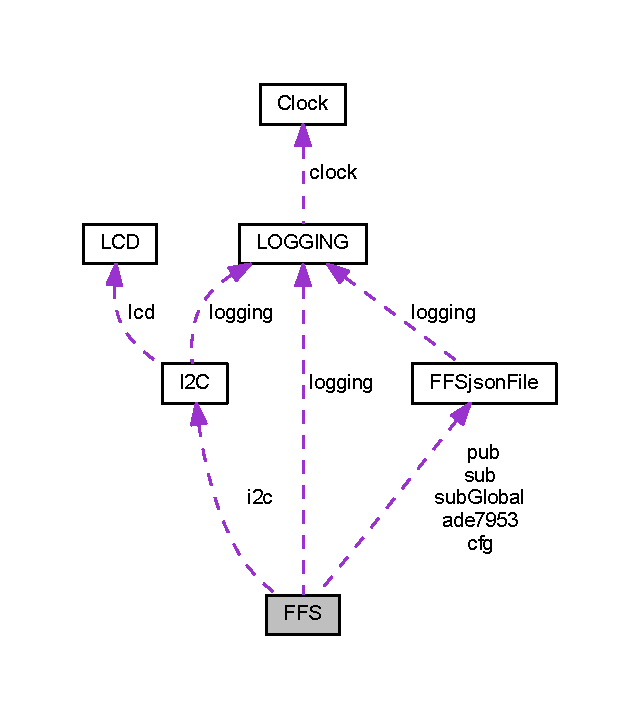
\includegraphics[width=307pt]{class_f_f_s__coll__graph}
\end{center}
\end{figure}
\subsection*{Öffentliche Methoden}
\begin{DoxyCompactItemize}
\item 
\mbox{\Hypertarget{class_f_f_s_abe1095a504fbac291132b6e953fafa77}\label{class_f_f_s_abe1095a504fbac291132b6e953fafa77}} 
{\bfseries F\+FS} (\hyperlink{class_l_o_g_g_i_n_g}{L\+O\+G\+G\+I\+NG} \&logging, \hyperlink{class_i2_c}{I2C} \&i2c)
\item 
\mbox{\Hypertarget{class_f_f_s_a4f3cd84efbb1cfb7e32782d11cedf803}\label{class_f_f_s_a4f3cd84efbb1cfb7e32782d11cedf803}} 
void {\bfseries mount} ()
\item 
\mbox{\Hypertarget{class_f_f_s_afb78519dca9d5f550b6f786de3dc1eac}\label{class_f_f_s_afb78519dca9d5f550b6f786de3dc1eac}} 
String {\bfseries load\+String} (String file\+Path)
\item 
\mbox{\Hypertarget{class_f_f_s_a26e3c3d788b8b225ce2095d1e7d3bf44}\label{class_f_f_s_a26e3c3d788b8b225ce2095d1e7d3bf44}} 
bool {\bfseries is\+Valid\+Json} (String root)
\item 
\mbox{\Hypertarget{class_f_f_s_a8fd9e800d2ca5643201d65338bf28b3d}\label{class_f_f_s_a8fd9e800d2ca5643201d65338bf28b3d}} 
String {\bfseries set} (\hyperlink{class_topic}{Topic} \&topic)
\item 
\mbox{\Hypertarget{class_f_f_s_a10ffd43fbbff003425dcbb76546b3518}\label{class_f_f_s_a10ffd43fbbff003425dcbb76546b3518}} 
String {\bfseries get} (\hyperlink{class_topic}{Topic} \&topic)
\end{DoxyCompactItemize}
\subsection*{Öffentliche Attribute}
\begin{DoxyCompactItemize}
\item 
\mbox{\Hypertarget{class_f_f_s_a5bf7b746aeb7ee29a3b3081984ca4f7c}\label{class_f_f_s_a5bf7b746aeb7ee29a3b3081984ca4f7c}} 
\hyperlink{class_l_o_g_g_i_n_g}{L\+O\+G\+G\+I\+NG} \& {\bfseries logging}
\item 
\mbox{\Hypertarget{class_f_f_s_a1d650679cb122fe7ee3b41e3deeae8f8}\label{class_f_f_s_a1d650679cb122fe7ee3b41e3deeae8f8}} 
\hyperlink{class_i2_c}{I2C} \& {\bfseries i2c}
\item 
\mbox{\Hypertarget{class_f_f_s_a82ef3f922de536af2d8d5317ea130a06}\label{class_f_f_s_a82ef3f922de536af2d8d5317ea130a06}} 
\hyperlink{class_f_f_sjson_file}{F\+F\+Sjson\+File} {\bfseries cfg}
\item 
\mbox{\Hypertarget{class_f_f_s_afe0bcfe44bc83bc1f7ea920303309344}\label{class_f_f_s_afe0bcfe44bc83bc1f7ea920303309344}} 
\hyperlink{class_f_f_sjson_file}{F\+F\+Sjson\+File} {\bfseries sub}
\item 
\mbox{\Hypertarget{class_f_f_s_ab718995f300e50922f3e5ea61169ae12}\label{class_f_f_s_ab718995f300e50922f3e5ea61169ae12}} 
\hyperlink{class_f_f_sjson_file}{F\+F\+Sjson\+File} {\bfseries sub\+Global}
\item 
\mbox{\Hypertarget{class_f_f_s_ac5412e6cd8a38c3c2ba5505a1827dfa2}\label{class_f_f_s_ac5412e6cd8a38c3c2ba5505a1827dfa2}} 
\hyperlink{class_f_f_sjson_file}{F\+F\+Sjson\+File} {\bfseries pub}
\item 
\mbox{\Hypertarget{class_f_f_s_afbe0842ffc05f157c3e23e907276d655}\label{class_f_f_s_afbe0842ffc05f157c3e23e907276d655}} 
\hyperlink{class_f_f_sjson_file}{F\+F\+Sjson\+File} {\bfseries ade7953}
\end{DoxyCompactItemize}


Die Dokumentation für diese Klasse wurde erzeugt aufgrund der Dateien\+:\begin{DoxyCompactItemize}
\item 
C\+:/\+T\+E\+M\+P/\+A\+D\+E7953-\/\+Power\+Socket/src/F\+F\+S.\+h\item 
C\+:/\+T\+E\+M\+P/\+A\+D\+E7953-\/\+Power\+Socket/src/F\+F\+S.\+cpp\end{DoxyCompactItemize}

\hypertarget{class_f_f_sjson_file}{}\section{F\+F\+Sjson\+File Klassenreferenz}
\label{class_f_f_sjson_file}\index{F\+F\+Sjson\+File@{F\+F\+Sjson\+File}}


Zusammengehörigkeiten von F\+F\+Sjson\+File\+:
\nopagebreak
\begin{figure}[H]
\begin{center}
\leavevmode
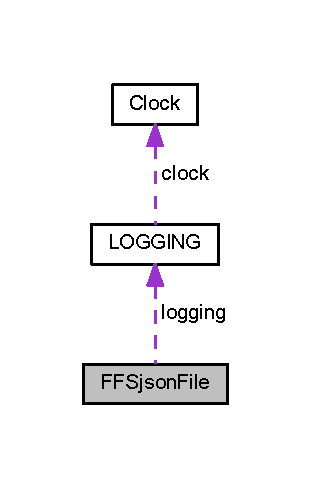
\includegraphics[width=149pt]{class_f_f_sjson_file__coll__graph}
\end{center}
\end{figure}
\subsection*{Öffentliche Methoden}
\begin{DoxyCompactItemize}
\item 
\mbox{\Hypertarget{class_f_f_sjson_file_aa4393b7da47cccc2a814c1341cff4955}\label{class_f_f_sjson_file_aa4393b7da47cccc2a814c1341cff4955}} 
{\bfseries F\+F\+Sjson\+File} (\hyperlink{class_l_o_g_g_i_n_g}{L\+O\+G\+G\+I\+NG} \&logging, String file\+Path, int type)
\item 
\mbox{\Hypertarget{class_f_f_sjson_file_a401e5929ca848aebeec6b32ef8a78383}\label{class_f_f_sjson_file_a401e5929ca848aebeec6b32ef8a78383}} 
void {\bfseries load\+File} ()
\item 
\mbox{\Hypertarget{class_f_f_sjson_file_a9a0f18ad2d55bcffb605d66a47d212d3}\label{class_f_f_sjson_file_a9a0f18ad2d55bcffb605d66a47d212d3}} 
String {\bfseries read\+Item} (String item\+Name)
\item 
\mbox{\Hypertarget{class_f_f_sjson_file_a1063b4ab2e854c77e5f8080b62c4f6de}\label{class_f_f_sjson_file_a1063b4ab2e854c77e5f8080b62c4f6de}} 
String {\bfseries read\+Item} (int item)
\item 
\mbox{\Hypertarget{class_f_f_sjson_file_a3fb3b4ff7dbfb9e52d11af0047bdce1f}\label{class_f_f_sjson_file_a3fb3b4ff7dbfb9e52d11af0047bdce1f}} 
bool {\bfseries write\+Item} (String item\+Name, String value)
\item 
\mbox{\Hypertarget{class_f_f_sjson_file_a157ab2e2736a52931ded20986af0f46a}\label{class_f_f_sjson_file_a157ab2e2736a52931ded20986af0f46a}} 
bool {\bfseries save\+File} ()
\end{DoxyCompactItemize}
\subsection*{Öffentliche Attribute}
\begin{DoxyCompactItemize}
\item 
\mbox{\Hypertarget{class_f_f_sjson_file_aa15032daa3d7179403433f72e1e1a657}\label{class_f_f_sjson_file_aa15032daa3d7179403433f72e1e1a657}} 
String {\bfseries file\+Path}
\item 
\mbox{\Hypertarget{class_f_f_sjson_file_a63bbb2a22adc5b918b48f6098d903b3f}\label{class_f_f_sjson_file_a63bbb2a22adc5b918b48f6098d903b3f}} 
\hyperlink{class_l_o_g_g_i_n_g}{L\+O\+G\+G\+I\+NG} \& {\bfseries logging}
\item 
\mbox{\Hypertarget{class_f_f_sjson_file_a4d0825acc72064f5ec0319141d41d16c}\label{class_f_f_sjson_file_a4d0825acc72064f5ec0319141d41d16c}} 
size\+\_\+t {\bfseries size}
\item 
\mbox{\Hypertarget{class_f_f_sjson_file_ac5f1818d70092331ece9c6601bed3e32}\label{class_f_f_sjson_file_ac5f1818d70092331ece9c6601bed3e32}} 
int {\bfseries items\+Count}
\item 
\mbox{\Hypertarget{class_f_f_sjson_file_ae56ea669e23c33baf323decf44de3a68}\label{class_f_f_sjson_file_ae56ea669e23c33baf323decf44de3a68}} 
int {\bfseries type}
\item 
\mbox{\Hypertarget{class_f_f_sjson_file_a9d474a402bf84b215c5203aa3152af62}\label{class_f_f_sjson_file_a9d474a402bf84b215c5203aa3152af62}} 
String {\bfseries root}
\end{DoxyCompactItemize}


Die Dokumentation für diese Klasse wurde erzeugt aufgrund der Dateien\+:\begin{DoxyCompactItemize}
\item 
C\+:/\+T\+E\+M\+P/\+A\+D\+E7953-\/\+Power\+Socket/src/F\+F\+S.\+h\item 
C\+:/\+T\+E\+M\+P/\+A\+D\+E7953-\/\+Power\+Socket/src/F\+F\+S.\+cpp\end{DoxyCompactItemize}

\hypertarget{class_f_f_sstring_file}{}\section{F\+F\+Sstring\+File Klassenreferenz}
\label{class_f_f_sstring_file}\index{F\+F\+Sstring\+File@{F\+F\+Sstring\+File}}


Zusammengehörigkeiten von F\+F\+Sstring\+File\+:
\nopagebreak
\begin{figure}[H]
\begin{center}
\leavevmode
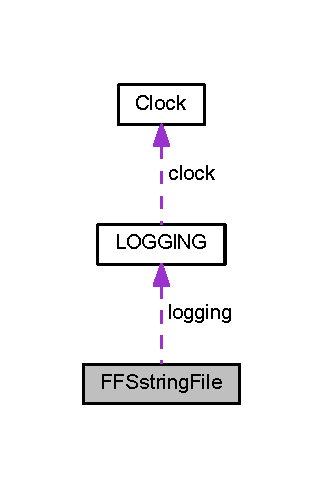
\includegraphics[width=155pt]{class_f_f_sstring_file__coll__graph}
\end{center}
\end{figure}
\subsection*{Öffentliche Methoden}
\begin{DoxyCompactItemize}
\item 
\mbox{\Hypertarget{class_f_f_sstring_file_aa5d7d691833c08b78a6fe1417bc405b7}\label{class_f_f_sstring_file_aa5d7d691833c08b78a6fe1417bc405b7}} 
{\bfseries F\+F\+Sstring\+File} (\hyperlink{class_l_o_g_g_i_n_g}{L\+O\+G\+G\+I\+NG} \&logging, String file\+Path)
\item 
\mbox{\Hypertarget{class_f_f_sstring_file_a4ba9dc7c294994f6530475a6b5748ca5}\label{class_f_f_sstring_file_a4ba9dc7c294994f6530475a6b5748ca5}} 
void {\bfseries load\+File} ()
\item 
\mbox{\Hypertarget{class_f_f_sstring_file_a83bdfffdcd8db1c924402997c0ed5b4e}\label{class_f_f_sstring_file_a83bdfffdcd8db1c924402997c0ed5b4e}} 
String {\bfseries read} ()
\end{DoxyCompactItemize}
\subsection*{Öffentliche Attribute}
\begin{DoxyCompactItemize}
\item 
\mbox{\Hypertarget{class_f_f_sstring_file_aefe29a42415aeb8cbe9e3895df3af963}\label{class_f_f_sstring_file_aefe29a42415aeb8cbe9e3895df3af963}} 
String {\bfseries file\+Path}
\item 
\mbox{\Hypertarget{class_f_f_sstring_file_a66b9cd649f3156cfe6287a97904ee0d0}\label{class_f_f_sstring_file_a66b9cd649f3156cfe6287a97904ee0d0}} 
\hyperlink{class_l_o_g_g_i_n_g}{L\+O\+G\+G\+I\+NG} \& {\bfseries logging}
\item 
\mbox{\Hypertarget{class_f_f_sstring_file_afa75bd6ea7c9a0cfbe1d5956c340c603}\label{class_f_f_sstring_file_afa75bd6ea7c9a0cfbe1d5956c340c603}} 
String {\bfseries data}
\end{DoxyCompactItemize}


Die Dokumentation für diese Klasse wurde erzeugt aufgrund der Dateien\+:\begin{DoxyCompactItemize}
\item 
C\+:/\+T\+E\+M\+P/\+A\+D\+E7953-\/\+Power\+Socket/src/F\+F\+S.\+h\item 
C\+:/\+T\+E\+M\+P/\+A\+D\+E7953-\/\+Power\+Socket/src/F\+F\+S.\+cpp\end{DoxyCompactItemize}

\hypertarget{class_i2_c}{}\section{I2C Klassenreferenz}
\label{class_i2_c}\index{I2C@{I2C}}


Zusammengehörigkeiten von I2C\+:
\nopagebreak
\begin{figure}[H]
\begin{center}
\leavevmode
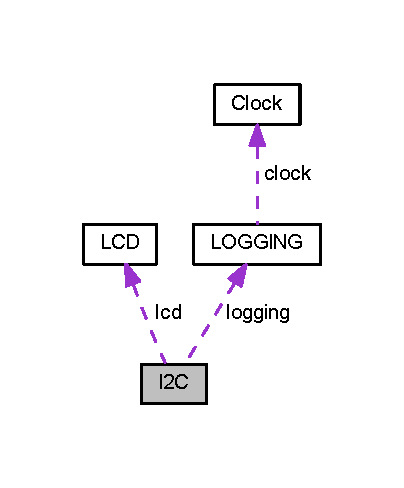
\includegraphics[width=194pt]{class_i2_c__coll__graph}
\end{center}
\end{figure}
\subsection*{Öffentliche Methoden}
\begin{DoxyCompactItemize}
\item 
\mbox{\Hypertarget{class_i2_c_a54577068652b30b6031442a28fa9a25b}\label{class_i2_c_a54577068652b30b6031442a28fa9a25b}} 
{\bfseries I2C} (\hyperlink{class_l_o_g_g_i_n_g}{L\+O\+G\+G\+I\+NG} \&logging)
\item 
\mbox{\Hypertarget{class_i2_c_a07463a2babdabbd675a2745fb53650ca}\label{class_i2_c_a07463a2babdabbd675a2745fb53650ca}} 
void {\bfseries start} ()
\item 
\mbox{\Hypertarget{class_i2_c_aa38babf0746e63bc9414ec0665f15b32}\label{class_i2_c_aa38babf0746e63bc9414ec0665f15b32}} 
void {\bfseries scan\+Bus} ()
\end{DoxyCompactItemize}
\subsection*{Öffentliche Attribute}
\begin{DoxyCompactItemize}
\item 
\mbox{\Hypertarget{class_i2_c_a8a905521f58afc3afb0ec9fd80f38c27}\label{class_i2_c_a8a905521f58afc3afb0ec9fd80f38c27}} 
\hyperlink{class_l_o_g_g_i_n_g}{L\+O\+G\+G\+I\+NG} \& {\bfseries logging}
\item 
\mbox{\Hypertarget{class_i2_c_afc1d2f3b9b877ce0db0e02a7ea85d42b}\label{class_i2_c_afc1d2f3b9b877ce0db0e02a7ea85d42b}} 
\hyperlink{class_l_c_d}{L\+CD} {\bfseries lcd}
\end{DoxyCompactItemize}


Die Dokumentation für diese Klasse wurde erzeugt aufgrund der Dateien\+:\begin{DoxyCompactItemize}
\item 
C\+:/\+T\+E\+M\+P/\+A\+D\+E7953-\/\+Power\+Socket/src/I2\+C.\+h\item 
C\+:/\+T\+E\+M\+P/\+A\+D\+E7953-\/\+Power\+Socket/src/I2\+C.\+cpp\end{DoxyCompactItemize}

\hypertarget{class_l_c_d}{}\section{L\+CD Klassenreferenz}
\label{class_l_c_d}\index{L\+CD@{L\+CD}}
\subsection*{Öffentliche Methoden}
\begin{DoxyCompactItemize}
\item 
\mbox{\Hypertarget{class_l_c_d_a1c9a188830514801292eb9972ef5ef36}\label{class_l_c_d_a1c9a188830514801292eb9972ef5ef36}} 
void {\bfseries init} ()
\item 
\mbox{\Hypertarget{class_l_c_d_a7514ab03fc96435731dccf816f90f460}\label{class_l_c_d_a7514ab03fc96435731dccf816f90f460}} 
void {\bfseries println} (String txt, const char $\ast$font\+Data, int y\+Pos)
\item 
\mbox{\Hypertarget{class_l_c_d_afa699e0beeeee03cce8cef87eba81c4a}\label{class_l_c_d_afa699e0beeeee03cce8cef87eba81c4a}} 
void {\bfseries clear} ()
\end{DoxyCompactItemize}


Die Dokumentation für diese Klasse wurde erzeugt aufgrund der Dateien\+:\begin{DoxyCompactItemize}
\item 
C\+:/\+T\+E\+M\+P/\+A\+D\+E7953-\/\+Power\+Socket/src/I2\+C.\+h\item 
C\+:/\+T\+E\+M\+P/\+A\+D\+E7953-\/\+Power\+Socket/src/I2\+C.\+cpp\end{DoxyCompactItemize}

\hypertarget{class_l_o_g_g_i_n_g}{}\section{L\+O\+G\+G\+I\+NG Klassenreferenz}
\label{class_l_o_g_g_i_n_g}\index{L\+O\+G\+G\+I\+NG@{L\+O\+G\+G\+I\+NG}}


Zusammengehörigkeiten von L\+O\+G\+G\+I\+NG\+:
\nopagebreak
\begin{figure}[H]
\begin{center}
\leavevmode
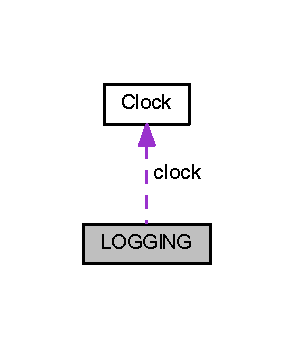
\includegraphics[width=141pt]{class_l_o_g_g_i_n_g__coll__graph}
\end{center}
\end{figure}
\subsection*{Öffentliche Methoden}
\begin{DoxyCompactItemize}
\item 
\mbox{\Hypertarget{class_l_o_g_g_i_n_g_a564b401f4aa450d865223b9a5c4c8c60}\label{class_l_o_g_g_i_n_g_a564b401f4aa450d865223b9a5c4c8c60}} 
{\bfseries L\+O\+G\+G\+I\+NG} (\hyperlink{class_clock}{Clock} \&clock)
\item 
\mbox{\Hypertarget{class_l_o_g_g_i_n_g_a79b6818ba95833469ed99f0d7ba7cf74}\label{class_l_o_g_g_i_n_g_a79b6818ba95833469ed99f0d7ba7cf74}} 
void {\bfseries start} ()
\item 
\mbox{\Hypertarget{class_l_o_g_g_i_n_g_a180904184ab56e7673643878223b87bb}\label{class_l_o_g_g_i_n_g_a180904184ab56e7673643878223b87bb}} 
void {\bfseries log} (const String \&channel, const String \&msg)
\item 
\mbox{\Hypertarget{class_l_o_g_g_i_n_g_a2dc3d19674867ddcf69ff3326ddd2059}\label{class_l_o_g_g_i_n_g_a2dc3d19674867ddcf69ff3326ddd2059}} 
void {\bfseries info} (const String \&msg)
\item 
\mbox{\Hypertarget{class_l_o_g_g_i_n_g_a20592566f7123f4027c814fd77edeb8d}\label{class_l_o_g_g_i_n_g_a20592566f7123f4027c814fd77edeb8d}} 
void {\bfseries error} (const String \&msg)
\item 
\mbox{\Hypertarget{class_l_o_g_g_i_n_g_a42b38c28ff116505e20d154507abfb06}\label{class_l_o_g_g_i_n_g_a42b38c28ff116505e20d154507abfb06}} 
void {\bfseries debug} (const String \&msg)
\end{DoxyCompactItemize}
\subsection*{Öffentliche Attribute}
\begin{DoxyCompactItemize}
\item 
\mbox{\Hypertarget{class_l_o_g_g_i_n_g_a7d93954ed4981f9309f69b09bd5a54ff}\label{class_l_o_g_g_i_n_g_a7d93954ed4981f9309f69b09bd5a54ff}} 
\hyperlink{class_clock}{Clock} \& {\bfseries clock}
\end{DoxyCompactItemize}


Die Dokumentation für diese Klasse wurde erzeugt aufgrund der Dateien\+:\begin{DoxyCompactItemize}
\item 
C\+:/\+T\+E\+M\+P/\+A\+D\+E7953-\/\+Power\+Socket/src/Logger.\+h\item 
C\+:/\+T\+E\+M\+P/\+A\+D\+E7953-\/\+Power\+Socket/src/Logger.\+cpp\end{DoxyCompactItemize}

\hypertarget{class_m_q_t_t}{}\section{M\+Q\+TT Klassenreferenz}
\label{class_m_q_t_t}\index{M\+Q\+TT@{M\+Q\+TT}}


Zusammengehörigkeiten von M\+Q\+TT\+:\nopagebreak
\begin{figure}[H]
\begin{center}
\leavevmode
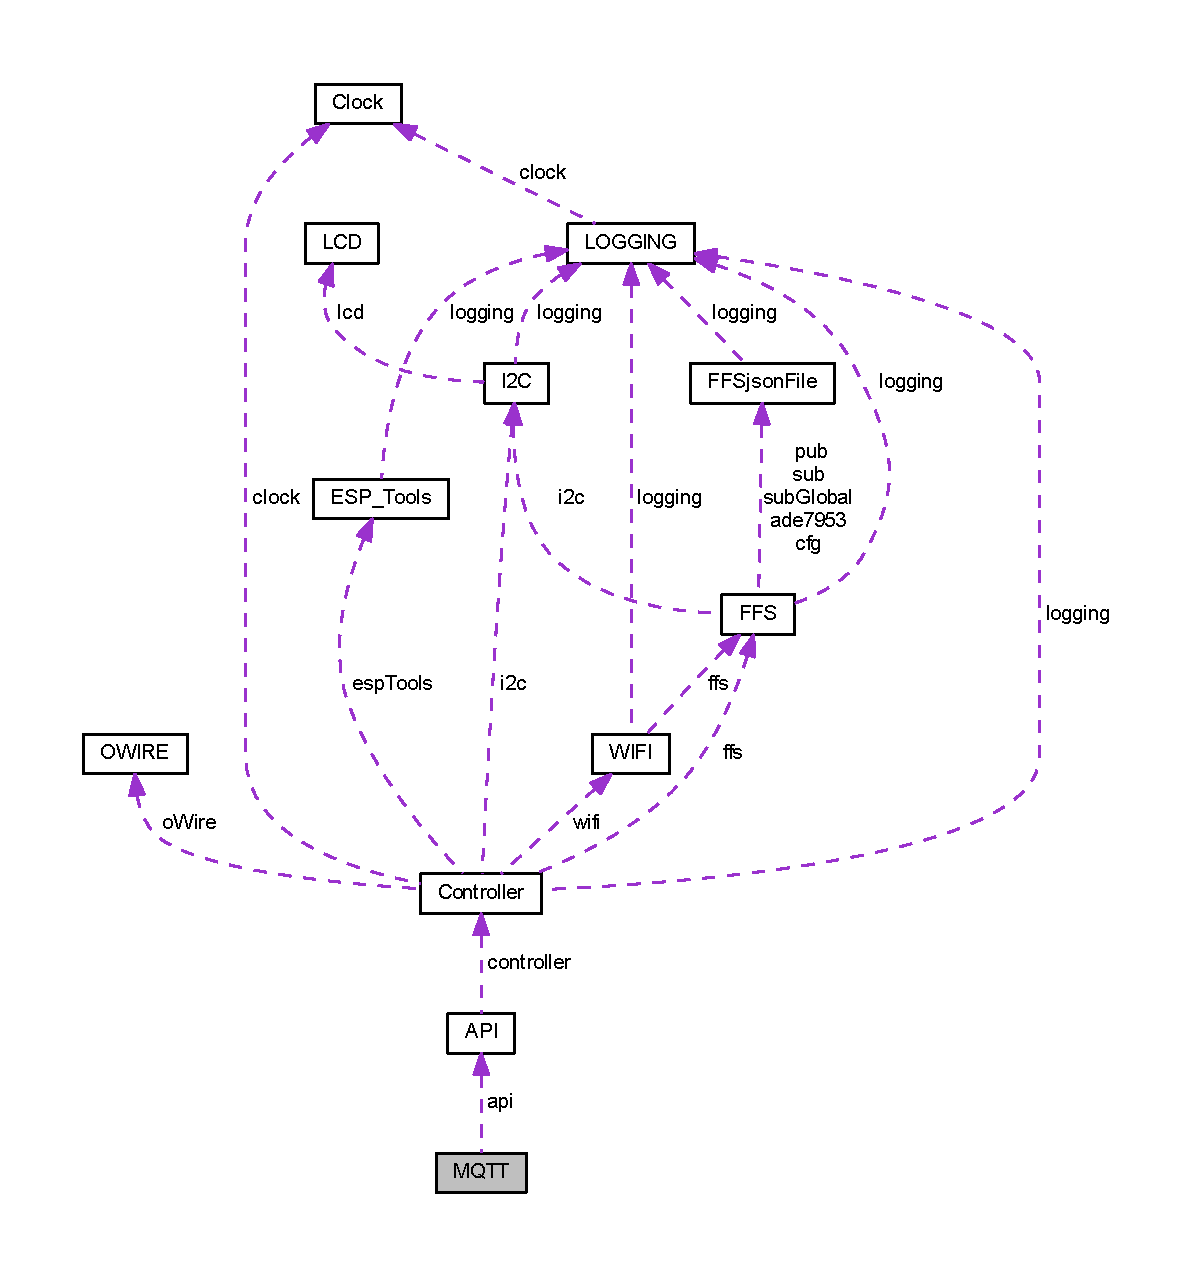
\includegraphics[width=350pt]{class_m_q_t_t__coll__graph}
\end{center}
\end{figure}
\subsection*{Öffentliche Methoden}
\begin{DoxyCompactItemize}
\item 
\mbox{\Hypertarget{class_m_q_t_t_a5908a8a2507409f065e9d68c4f086f91}\label{class_m_q_t_t_a5908a8a2507409f065e9d68c4f086f91}} 
{\bfseries M\+Q\+TT} (\hyperlink{class_a_p_i}{A\+PI} \&api)
\item 
\mbox{\Hypertarget{class_m_q_t_t_ae15d841989b9faa5b93a2682b8b92bbb}\label{class_m_q_t_t_ae15d841989b9faa5b93a2682b8b92bbb}} 
bool {\bfseries start} ()
\item 
\mbox{\Hypertarget{class_m_q_t_t_a14be943e1a3441660f2a6c86ffeed6a4}\label{class_m_q_t_t_a14be943e1a3441660f2a6c86ffeed6a4}} 
bool {\bfseries handle} ()
\item 
\mbox{\Hypertarget{class_m_q_t_t_aa518d3877c2a6cd83e5e4ade22b9226f}\label{class_m_q_t_t_aa518d3877c2a6cd83e5e4ade22b9226f}} 
void {\bfseries set\+Callback} (M\+Q\+T\+T\+\_\+\+C\+A\+L\+L\+B\+A\+C\+K\+\_\+\+S\+I\+G\+N\+A\+T\+U\+RE)
\item 
\mbox{\Hypertarget{class_m_q_t_t_a1b777cfb8d300947e1f5b35c0d18cf47}\label{class_m_q_t_t_a1b777cfb8d300947e1f5b35c0d18cf47}} 
void {\bfseries on\+\_\+incomming\+Subcribe} (char $\ast$topic, byte $\ast$payload, unsigned int length)
\item 
\mbox{\Hypertarget{class_m_q_t_t_af0666c91c7c9b6ed6504107f5197c4f3}\label{class_m_q_t_t_af0666c91c7c9b6ed6504107f5197c4f3}} 
void {\bfseries pub} (String topic, String value)
\end{DoxyCompactItemize}
\subsection*{Öffentliche Attribute}
\begin{DoxyCompactItemize}
\item 
\mbox{\Hypertarget{class_m_q_t_t_a2ca668403e3068d75e85749151904a5e}\label{class_m_q_t_t_a2ca668403e3068d75e85749151904a5e}} 
\hyperlink{class_a_p_i}{A\+PI} \& {\bfseries api}
\end{DoxyCompactItemize}


Die Dokumentation für diese Klasse wurde erzeugt aufgrund der Dateien\+:\begin{DoxyCompactItemize}
\item 
C\+:/\+T\+E\+M\+P/\+A\+D\+E7953-\/\+Power\+Socket/src/M\+Q\+T\+T.\+h\item 
C\+:/\+T\+E\+M\+P/\+A\+D\+E7953-\/\+Power\+Socket/src/M\+Q\+T\+T.\+cpp\end{DoxyCompactItemize}

\hypertarget{class_o_w_i_r_e}{}\section{O\+W\+I\+RE Klassenreferenz}
\label{class_o_w_i_r_e}\index{O\+W\+I\+RE@{O\+W\+I\+RE}}


Die Dokumentation für diese Klasse wurde erzeugt aufgrund der Dateien\+:\begin{DoxyCompactItemize}
\item 
C\+:/\+T\+E\+M\+P/\+A\+D\+E7953-\/\+Power\+Socket/src/o\+Wire.\+h\item 
C\+:/\+T\+E\+M\+P/\+A\+D\+E7953-\/\+Power\+Socket/src/o\+Wire.\+cpp\end{DoxyCompactItemize}

\hypertarget{class_session}{}\section{Session Klassenreferenz}
\label{class_session}\index{Session@{Session}}
\subsection*{Öffentliche Methoden}
\begin{DoxyCompactItemize}
\item 
\mbox{\Hypertarget{class_session_a7f2713b9d3b5284c50fe2e1b4737afb1}\label{class_session_a7f2713b9d3b5284c50fe2e1b4737afb1}} 
{\bfseries Session} (String username, \hyperlink{class_a_p_i}{A\+PI} \&api)
\item 
\mbox{\Hypertarget{class_session_a8a1e5f5100ffaba505d173b76cad19a4}\label{class_session_a8a1e5f5100ffaba505d173b76cad19a4}} 
String {\bfseries get\+Session\+Id} ()
\item 
\mbox{\Hypertarget{class_session_aee582a7f3e3f09d4b7f1f7bcdb39a1b2}\label{class_session_aee582a7f3e3f09d4b7f1f7bcdb39a1b2}} 
String {\bfseries get\+Username} ()
\item 
\mbox{\Hypertarget{class_session_a65cba5b1fba90e243099779ffa776a21}\label{class_session_a65cba5b1fba90e243099779ffa776a21}} 
bool {\bfseries is\+Expired} ()
\item 
\mbox{\Hypertarget{class_session_aecd99d82f2905578d1492de00dcc9aa9}\label{class_session_aecd99d82f2905578d1492de00dcc9aa9}} 
void {\bfseries touch} ()
\end{DoxyCompactItemize}


Die Dokumentation für diese Klasse wurde erzeugt aufgrund der Dateien\+:\begin{DoxyCompactItemize}
\item 
C\+:/\+T\+E\+M\+P/\+A\+D\+E7953-\/\+Power\+Socket/src/Auth.\+h\item 
C\+:/\+T\+E\+M\+P/\+A\+D\+E7953-\/\+Power\+Socket/src/Auth.\+cpp\end{DoxyCompactItemize}

\hypertarget{class_sys_utils}{}\section{Sys\+Utils Klassenreferenz}
\label{class_sys_utils}\index{Sys\+Utils@{Sys\+Utils}}
\subsection*{Öffentliche, statische Methoden}
\begin{DoxyCompactItemize}
\item 
\mbox{\Hypertarget{class_sys_utils_a50dac2b668ef371816e5a1e304079a58}\label{class_sys_utils_a50dac2b668ef371816e5a1e304079a58}} 
static long {\bfseries rand} (long max)
\item 
\mbox{\Hypertarget{class_sys_utils_a4bc82b33a63dcc0ae82ebef407597f98}\label{class_sys_utils_a4bc82b33a63dcc0ae82ebef407597f98}} 
static I\+P\+Address {\bfseries char\+To\+IP} (char $\ast$IP)
\item 
\mbox{\Hypertarget{class_sys_utils_a44dcc4af3a7b24cda66b631f143091e5}\label{class_sys_utils_a44dcc4af3a7b24cda66b631f143091e5}} 
static I\+P\+Address {\bfseries str\+To\+IP} (String IP)
\item 
\mbox{\Hypertarget{class_sys_utils_aac2eed5ca71ab6c90961e6c53c4f871b}\label{class_sys_utils_aac2eed5ca71ab6c90961e6c53c4f871b}} 
static char $\ast$ {\bfseries string2char} (String command)
\item 
\mbox{\Hypertarget{class_sys_utils_a02d7d2d29d456083b5df9ab732ef7682}\label{class_sys_utils_a02d7d2d29d456083b5df9ab732ef7682}} 
static String {\bfseries str\+Date} (time\+\_\+t t)
\item 
\mbox{\Hypertarget{class_sys_utils_ab0a24909211407b58a8400b22ae95db5}\label{class_sys_utils_ab0a24909211407b58a8400b22ae95db5}} 
static String {\bfseries str\+Time} (time\+\_\+t t)
\item 
\mbox{\Hypertarget{class_sys_utils_a64f16b8c4cdde00cb9bcab6de4e5ceb4}\label{class_sys_utils_a64f16b8c4cdde00cb9bcab6de4e5ceb4}} 
static String {\bfseries str\+Time\+\_\+ms} (time\+\_\+t t)
\item 
\mbox{\Hypertarget{class_sys_utils_a32700011267ea8e220e0e648f5e4f014}\label{class_sys_utils_a32700011267ea8e220e0e648f5e4f014}} 
static String {\bfseries str\+Date\+Time} (time\+\_\+t t)
\item 
\mbox{\Hypertarget{class_sys_utils_a042a58a4c1115579c9a7e10f5d1d15f1}\label{class_sys_utils_a042a58a4c1115579c9a7e10f5d1d15f1}} 
static String {\bfseries str\+Date\+Time\+\_\+ms} (time\+\_\+t t)
\end{DoxyCompactItemize}
\subsection*{Statische öffentliche Attribute}
\begin{DoxyCompactItemize}
\item 
\mbox{\Hypertarget{class_sys_utils_a9419bcdbf1047a6aa8b92361416c1d75}\label{class_sys_utils_a9419bcdbf1047a6aa8b92361416c1d75}} 
static long {\bfseries seed} = 0
\end{DoxyCompactItemize}


Die Dokumentation für diese Klasse wurde erzeugt aufgrund der Dateien\+:\begin{DoxyCompactItemize}
\item 
C\+:/\+T\+E\+M\+P/\+A\+D\+E7953-\/\+Power\+Socket/src/Sys\+Utils.\+h\item 
C\+:/\+T\+E\+M\+P/\+A\+D\+E7953-\/\+Power\+Socket/src/Sys\+Utils.\+cpp\end{DoxyCompactItemize}

\hypertarget{class_topic}{}\section{Topic Klassenreferenz}
\label{class_topic}\index{Topic@{Topic}}
\subsection*{Öffentliche Methoden}
\begin{DoxyCompactItemize}
\item 
\mbox{\Hypertarget{class_topic_a0a440ad48222b711fc0568bb66bbcf64}\label{class_topic_a0a440ad48222b711fc0568bb66bbcf64}} 
{\bfseries Topic} (String \&topics\+Args)
\item 
\mbox{\Hypertarget{class_topic_a9288183546263ded5b071462c9515f71}\label{class_topic_a9288183546263ded5b071462c9515f71}} 
{\bfseries Topic} (char $\ast$topics, char $\ast$args)
\item 
\mbox{\Hypertarget{class_topic_a08531a42771dcb911dcf800feb5623fb}\label{class_topic_a08531a42771dcb911dcf800feb5623fb}} 
String {\bfseries topic\+\_\+as\+String} ()
\item 
\mbox{\Hypertarget{class_topic_a0de810b3f2179e9f13dbe34029e5dafe}\label{class_topic_a0de810b3f2179e9f13dbe34029e5dafe}} 
String {\bfseries arg\+\_\+as\+String} ()
\item 
\mbox{\Hypertarget{class_topic_a19bdafb2d4bb697323cc51999715436d}\label{class_topic_a19bdafb2d4bb697323cc51999715436d}} 
String {\bfseries as\+String} ()
\item 
\mbox{\Hypertarget{class_topic_a90ad578f6e8e61da6299052df5dc8c19}\label{class_topic_a90ad578f6e8e61da6299052df5dc8c19}} 
void {\bfseries dissect\+Topic} (char $\ast$topics, char $\ast$arg)
\item 
\mbox{\Hypertarget{class_topic_a3518620d9036102c1afb57877afa3883}\label{class_topic_a3518620d9036102c1afb57877afa3883}} 
String {\bfseries modify\+Topic} (int index)
\item 
\mbox{\Hypertarget{class_topic_ab0145e4229a16c728ddb5caa40b42120}\label{class_topic_ab0145e4229a16c728ddb5caa40b42120}} 
bool {\bfseries item\+Is} (int index, const string topic\+Name)
\end{DoxyCompactItemize}
\subsection*{Öffentliche Attribute}
\begin{DoxyCompactItemize}
\item 
\mbox{\Hypertarget{class_topic_a5734fadd98a2cce17238891a7910aef4}\label{class_topic_a5734fadd98a2cce17238891a7910aef4}} 
string $\ast$ {\bfseries item}
\item 
\mbox{\Hypertarget{class_topic_af5e7eb036a84af9515d1463152bf5a4c}\label{class_topic_af5e7eb036a84af9515d1463152bf5a4c}} 
string $\ast$ {\bfseries arg}
\item 
\mbox{\Hypertarget{class_topic_af6b484a1ad52debc304c84a53560a324}\label{class_topic_af6b484a1ad52debc304c84a53560a324}} 
char $\ast$ {\bfseries topics}
\item 
\mbox{\Hypertarget{class_topic_ab30006d032a999fa1c81653b1a6c956d}\label{class_topic_ab30006d032a999fa1c81653b1a6c956d}} 
char $\ast$ {\bfseries args}
\item 
\mbox{\Hypertarget{class_topic_a0051cfe99f9f26dcdb9b3480d186afd9}\label{class_topic_a0051cfe99f9f26dcdb9b3480d186afd9}} 
int {\bfseries count\+Items} = 0
\item 
\mbox{\Hypertarget{class_topic_ab85b1147f2b466a0cbe2dfed2d719fdd}\label{class_topic_ab85b1147f2b466a0cbe2dfed2d719fdd}} 
int {\bfseries count\+Args} = 0
\end{DoxyCompactItemize}


Die Dokumentation für diese Klasse wurde erzeugt aufgrund der Dateien\+:\begin{DoxyCompactItemize}
\item 
C\+:/\+T\+E\+M\+P/\+A\+D\+E7953-\/\+Power\+Socket/src/Topic.\+h\item 
C\+:/\+T\+E\+M\+P/\+A\+D\+E7953-\/\+Power\+Socket/src/Topic.\+cpp\end{DoxyCompactItemize}

\hypertarget{struct_t_topic}{}\section{T\+Topic Strukturreferenz}
\label{struct_t_topic}\index{T\+Topic@{T\+Topic}}


Die Dokumentation für diese Struktur wurde erzeugt aufgrund der Datei\+:\begin{DoxyCompactItemize}
\item 
C\+:/\+T\+E\+M\+P/\+A\+D\+E7953-\/\+Power\+Socket/src/Topic.\+h\end{DoxyCompactItemize}

\hypertarget{class_w_e_b_i_f}{}\section{W\+E\+B\+IF Klassenreferenz}
\label{class_w_e_b_i_f}\index{W\+E\+B\+IF@{W\+E\+B\+IF}}
\subsection*{Öffentliche Methoden}
\begin{DoxyCompactItemize}
\item 
\mbox{\Hypertarget{class_w_e_b_i_f_a8717e0a1ac2c54e3019c23decd22a94d}\label{class_w_e_b_i_f_a8717e0a1ac2c54e3019c23decd22a94d}} 
{\bfseries W\+E\+B\+IF} (\hyperlink{class_a_p_i}{A\+PI} \&api)
\item 
\mbox{\Hypertarget{class_w_e_b_i_f_a489fe1efb217ecedfe5391c71e9f8b4c}\label{class_w_e_b_i_f_a489fe1efb217ecedfe5391c71e9f8b4c}} 
void {\bfseries start} ()
\item 
\mbox{\Hypertarget{class_w_e_b_i_f_a88fc15cda66431436ea0de38a0d4c734}\label{class_w_e_b_i_f_a88fc15cda66431436ea0de38a0d4c734}} 
void {\bfseries handle} ()
\end{DoxyCompactItemize}


Die Dokumentation für diese Klasse wurde erzeugt aufgrund der Dateien\+:\begin{DoxyCompactItemize}
\item 
C\+:/\+T\+E\+M\+P/\+A\+D\+E7953-\/\+Power\+Socket/src/W\+E\+B\+Server.\+h\item 
C\+:/\+T\+E\+M\+P/\+A\+D\+E7953-\/\+Power\+Socket/src/W\+E\+B\+Server.\+cpp\end{DoxyCompactItemize}

\hypertarget{class_w_i_f_i}{}\section{W\+I\+FI Klassenreferenz}
\label{class_w_i_f_i}\index{W\+I\+FI@{W\+I\+FI}}


Zusammengehörigkeiten von W\+I\+FI\+:
\nopagebreak
\begin{figure}[H]
\begin{center}
\leavevmode
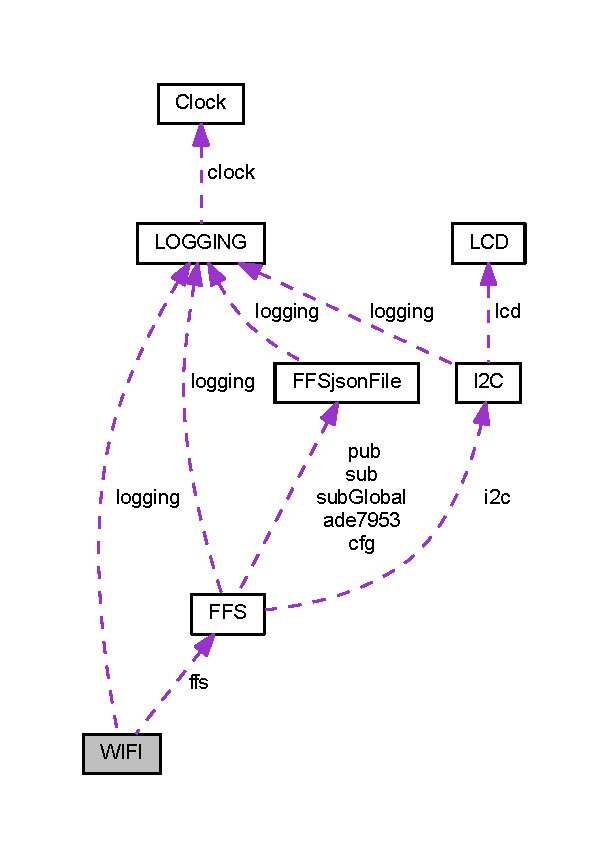
\includegraphics[width=292pt]{class_w_i_f_i__coll__graph}
\end{center}
\end{figure}
\subsection*{Öffentliche Methoden}
\begin{DoxyCompactItemize}
\item 
\mbox{\Hypertarget{class_w_i_f_i_afc734f0cace3978a3304c4b70a364f57}\label{class_w_i_f_i_afc734f0cace3978a3304c4b70a364f57}} 
{\bfseries W\+I\+FI} (\hyperlink{class_l_o_g_g_i_n_g}{L\+O\+G\+G\+I\+NG} \&logging, \hyperlink{class_f_f_s}{F\+FS} \&ffs)
\item 
\mbox{\Hypertarget{class_w_i_f_i_a554751a46e587d8952e9792fb2b8d1f1}\label{class_w_i_f_i_a554751a46e587d8952e9792fb2b8d1f1}} 
void {\bfseries set\+\_\+callbacks} (Callback\+Function wifi\+Connected, Callback\+Function wifi\+Disconnected)
\item 
\mbox{\Hypertarget{class_w_i_f_i_a890d05b9593104d9b9194e80e2229bdf}\label{class_w_i_f_i_a890d05b9593104d9b9194e80e2229bdf}} 
bool {\bfseries start} ()
\item 
\mbox{\Hypertarget{class_w_i_f_i_a5f31e525ef4009a1c375c51a57e6fddc}\label{class_w_i_f_i_a5f31e525ef4009a1c375c51a57e6fddc}} 
bool {\bfseries handle} ()
\item 
\mbox{\Hypertarget{class_w_i_f_i_a44bf4fdb6860bcc8c65559abfa779622}\label{class_w_i_f_i_a44bf4fdb6860bcc8c65559abfa779622}} 
String {\bfseries mac\+Address} ()
\item 
\mbox{\Hypertarget{class_w_i_f_i_a601248aeebafdf3581a33356e52d30f8}\label{class_w_i_f_i_a601248aeebafdf3581a33356e52d30f8}} 
String {\bfseries get} (\hyperlink{class_topic}{Topic} \&topic)
\end{DoxyCompactItemize}
\subsection*{Öffentliche Attribute}
\begin{DoxyCompactItemize}
\item 
\mbox{\Hypertarget{class_w_i_f_i_afd6bbf4f690b9758c300b3e4e0d1f294}\label{class_w_i_f_i_afd6bbf4f690b9758c300b3e4e0d1f294}} 
\hyperlink{class_l_o_g_g_i_n_g}{L\+O\+G\+G\+I\+NG} \& {\bfseries logging}
\item 
\mbox{\Hypertarget{class_w_i_f_i_af1e3a48cc5f0bd3c3ab3245279b7cef3}\label{class_w_i_f_i_af1e3a48cc5f0bd3c3ab3245279b7cef3}} 
\hyperlink{class_f_f_s}{F\+FS} \& {\bfseries ffs}
\item 
\mbox{\Hypertarget{class_w_i_f_i_a200fc29ce84c782a7eee94bf9b0d1660}\label{class_w_i_f_i_a200fc29ce84c782a7eee94bf9b0d1660}} 
Wi\+Fi\+Client {\bfseries client}
\item 
\mbox{\Hypertarget{class_w_i_f_i_ab619e6b80e554ca319808dfaf6eb82ba}\label{class_w_i_f_i_ab619e6b80e554ca319808dfaf6eb82ba}} 
bool {\bfseries Wi\+Fi\+Status} = false
\end{DoxyCompactItemize}


Die Dokumentation für diese Klasse wurde erzeugt aufgrund der Dateien\+:\begin{DoxyCompactItemize}
\item 
C\+:/\+T\+E\+M\+P/\+A\+D\+E7953-\/\+Power\+Socket/src/W\+I\+F\+I.\+h\item 
C\+:/\+T\+E\+M\+P/\+A\+D\+E7953-\/\+Power\+Socket/src/W\+I\+F\+I.\+cpp\end{DoxyCompactItemize}

%--- End generated contents ---

% Index
\backmatter
\newpage
\phantomsection
\clearemptydoublepage
\addcontentsline{toc}{chapter}{Index}
\printindex

\end{document}
